\documentclass[10pt, a4paper]{article}
\usepackage{verbatim}
\usepackage{textcomp}
\usepackage{amsmath}
\usepackage{graphicx}
\usepackage{import}
\usepackage{epstopdf}
\usepackage{subcaption}
\usepackage{caption}
\usepackage{tabularx}
\usepackage{booktabs}
\title{My \LaTeX{} Demos}
\author{Mustafa Can Yucel}
\begin{document}
\maketitle
\begin{abstract}
This is a sample document for demonstrating what I have learned during \LaTeX{} study. There are examples for styles, floating objects, commands and almost all other commonly used \LaTeX{}  properties and settings.

The environment used is MikTeX 2.9 and TexMaker and lately TexStudio. The current incarnation \LaTeXe{} is used as of \today.
\end{abstract}
\newpage
\tableofcontents
\newpage
\section{Things Needed to Know}
\subsection{Spaces}
White-space characters, whatever their numbers are, are treated as a single space. In this sentence, there are actually six spaces between two brackets:(      ). You see only one, right? Funny stuff.

An empty line in the code starts a new paragraph, such as this one.
\subsection{Special Characters}
The following symbols are reserved as they either have a special meaning in \LaTeX{}, or they are not available in all the fonts: \# \$ \% \^ \& \_ \{ \} \textbackslash

These can be used in text body by the escape character backslash. Backslash cannot be escaped by itself, so the command \textbackslash textbackslash is used: 
\begin{verbatim}
	\# \$ \% \^ \& \_ \{ \} \textbackslash
\end{verbatim}

\subsection{Comments}
\% is used for simple commenting:

This sentence %though stupid
%but still
has a comment in itself.

For longer comments, \textsl{comment} environment of verbatim package may be used.

This sentence also has a \begin{comment} still stupid,
but longer and more
structured \end{comment}
comment in it.
\begin{verbatim}
	This sentence %though stupid
	%but still
	has a comment in itself.
	
	For longer comments, \textsl{comment} environment of verbatim package may be used.
	
	This sentence also has a \begin{comment} still stupid,
	but longer and more
	structured \end{comment}
	comment in it.
\end{verbatim}
\subsection{Starting a New Page}
When we want to start a new page, there are several alternatives to be used.
\begin{description}
	\item[newpage] This command immediately ends the page, but does not process float queues. Therefore, if you have any floats in these lists, they will be put to the new page.
	\item[clearpage] It ends the current page and causes all figures and tables appeared so far in the input to be printed.
	\item[cleardoublepage] This also  ends the current page and causes all figures and tables appeared so far in the input to be printed. Moreover, in a two-sided printing style, it also makes the new page a right-hand (an odd-numbered) page, producing a blank page if necessary.
\end{description}
\clearpage
\section{Typesetting Text}
\subsection{Quotation Marks}
This is an example sentence to demonstrate `single' and ``double'' quotation marks. Opening mark is done by grave accent and closing mark is done by vertical quote:
\begin{verbatim}
	`single' vs ``double''
\end{verbatim}
\subsection{Degree Symbol}
Creating $\,^{\circ}\mathrm{C}$ by pure \LaTeX{} is complex. Creating \textcelsius{} by \texttt{textcomp} package is easy, though:
\begin{verbatim}
$\,^{\circ}\mathrm{C}$ versus \textcelsius
\end{verbatim}
\subsection{Ellipsis}
On a typewriter, period and comma have the same width with other characters. On a print, however, they are smaller and closer to the preceding character. Therefore, using three dots for `ellipsis' is not correct. The command \textbackslash\textsl{ldots} should be used:\\
This is ... not true.\\
This is \ldots true.
\begin{verbatim}
	This is ... not true.\\
	This is \ldots true.
\end{verbatim}
\subsection{Cross-References}
\textsl{label, ref, pageref} commands are used for cross referencing with a user defined marker string. \LaTeX{} replaces \textsl{ref} by the number of the section, subsection, figure, table or theorem after which the corresponding \textsl{label} command occurred. 
Another good point of \LaTeX{} is that you can easily reference almost anything that is numbered, and \LaTeX{} will take care of the numbering, updating it when necessary. The commands do not depend on environment to be referenced, it is just:
\begin{verbatim}
	\label{marker}
	...
	\ref{marker}
\end{verbatim}

The label \texttt{marker} will not be visible in the compiled product. \LaTeX{} will calculate the correct number for the objects in the document, and then it will replace the string \texttt{\textbackslash ref\{marker\}} with the right number that was assigned to the object. If a reference to a marker that does not exist is used, the document may or may not be compiled (TexStudio gives an error, but other programs may compile just giving a warning.). If compiled, unknown references will be shown as ``??'' in the PDF. 
As you may have guessed, compiling references is a two step process; first the compiler has to store the labels with the right numbering to be used for referencing. And then it has to replace all \texttt{\textbackslash ref} strings with the correct numbers. That's why compiling a document twice is required to update all the references when large changes are done in reference list. Some IDEs do this automatically (such as TexStudio), as if \LaTeX{} realizes references may have changed to require a second compilation, it throws a warning:
\begin{quote}
	\begin{verbatim}
		LaTeX Warning: Label(s) may have changed. Rerun to get 
		cross-references right.
	\end{verbatim}
\end{quote}

Using the command \texttt{\textbackslash pageref} returns the page of the referenced marker. 
A reference to this sub-section\label{this} looks like: ``see section \ref{this} on page \pageref{this}''.
\begin{verbatim}
	see section \ref{this} on page \pageref{this}
\end{verbatim}

Since the same command is used for every environment, it is customary to use conventional abbreviations for different types of labels:
\begin{table}[htbp]
	\centering
	\begin{tabular}{|c|c|}
	\hline fig: & Figure \\ 
	\hline sec: & Section \\ 
	\hline subsec: & Subsection \\ 
	\hline chap: & Chapter \\ 
	\hline tab: & Table \\ 
	\hline eq: & Equation \\ 
	\hline lst: & Code Listing \\ 
	\hline itm: & Enumerated List Item \\ 
	\hline app: & Appendix Subsection \\ 
	\hline 
\end{tabular} 
\end{table}

Some packages such as \textsl{fancyref} also rely on these meta data information. Another suggestion is to avoid numbering in label identifiers, as re-numbering will be required on most of the changes. 

Floats such as \texttt{table} or \texttt{figure} are NOT label-able. Therefore, they need a \textit{caption} element as an identifier. While referencing these environments, \texttt{\textbackslash label} command should be put after the \texttt{\textbackslash caption} element. To be completely safe, it could be put inside the \texttt{\textbackslash caption} element as well. If not put inside or after captions, reference commands will pick up the current section or list number instead of what you intended.

In case you use the package \textsl{hyperref} to create a PDF, the links to tables or figures will point to the caption of the table or figure, which is always below/above the table or figure itself. Therefore the table or figure will not be visible, if it is above the pointer and one has to scroll up in order to see it. If you want the link point to the top of the image you can give the option \texttt{hypcap} to the \textsl{caption} package:
\begin{verbatim}
	\usepackage[hypcap]{caption}
\end{verbatim}

Referencing equations is the same:
\begin{verbatim}
	\begin{equation} \label{eq:solve}
	x^2 - 5 x + 6 = 0
	\end{equation}
	\begin{equation}
	x_1 = \frac{5 + \sqrt{25 - 4 \times 6}}{2} = 3
	\end{equation}
	\begin{equation}
	x_2 = \frac{5 - \sqrt{25 - 4 \times 6}}{2} = 2
	\end{equation}
	
	and so we have solved equation ~\ref{eq:solve}
\end{verbatim}

The \textsl{amsmath} dds a new command for referencing formulae; it is \texttt{\textbackslash eqref}. It works exactly like \texttt{\textbackslash ref}, but it adds parentheses so that, instead of printing a plain number as 5, it will print (5). This can be useful to help the reader distinguish between formulae and other things, without the need to repeat the word "formula" before any reference. Its output can be changed as desired; for more information see the \textsl{amsmath} documentation.

The \textsl{amsmath} package also adds the \texttt{\textbackslash numberwithin\{countera\}\{counterb\}} command which replaces the simple countera by a more sophisticated counterb.countera. For example:
\begin{verbatim}
	\numberwithin{equation}{section} 
\end{verbatim} 
in the preamble will prepend the section number to all equation numbers.

The \textsl{cases} package adds the \texttt{\textbackslash numcases} and the \texttt{\textbackslash subnumcases} commands, which produce multi-case equations with a separate equation number and a separate equation number plus a letter, respectively, for each case.

The \textsl{hyperref} package introduces another useful command; \texttt{\textbackslash autoref\{\}}. This command creates a reference with additional text corresponding to the target's type, all of which will be a hyperlink. For example, the command \texttt{\textbackslash autoref\{sec:intro\}} would create a hyperlink to the \texttt{\textbackslash label\{sec:intro\}} command, wherever it is. Assuming that this label is pointing to a section, the hyperlink would contain the text "section 3.4", or similar.

When you define a \texttt{\textbackslash label} outside a figure, a table, or other floating objects, the label points to the current section. In some cases, this behavior is not what you'd like and you'd prefer the generated link to point to the line where the \texttt{\textbackslash label} is defined. This can be achieved with the command \texttt{\textbackslash phantomsection} as in this example:
\begin{verbatim}
	%The link location will be placed on the line below.
	\phantomsection
	\label{the_label}
\end{verbatim}
\subsection{Footnotes}
The command \textsl{footnote} is used. As an example this sentence\footnote{Yes, this one} has a footnote. 
\subsection{Emphasizing Words}
For the aim of emphasize, words can be \underline{underlined} or \emph{emphasized\footnote{Does not make sense, does it?}}:
\begin{verbatim}
\underline{underlined}
\emph{emphasized}
\end{verbatim}
\subsection{Environments}
Environments are defined between \textbackslash\textsl{begin} and \textbackslash\textsl{end} commands.

\subsubsection{Itemize, Enumerate, Description}
\emph{itemize} is used for simple lists, \emph{enumerate} for enumerated lists and \emph{description} for definitions:

\begin{enumerate}
\item List environments can be nested in any fashion:
\begin{itemize}
\item Still, after some level it looks silly
\item[-] with some special characters
\end{itemize}
\item Therefore remember:
\begin{description}
\item[Stupid] things will not be smart because they are in a list.
\item[Smart] things can be presented beautifully in lists.
\end{description}
\end{enumerate}

\begin{verbatim}
\begin{enumerate}
\item List environments can be nested in any fashion:
\begin{itemize}
\item Still, after some level it looks silly
\item[-] with some special characters
\end{itemize}
\item Therefore remember:
\begin{description}
\item[Stupid] things will not be smart because they are in a list.
\item[Smart] things can be presented beautifully in lists.
\end{description}
\end{enumerate}
\end{verbatim}

\subsubsection{Flushleft, Flushright and Center}
They generate paragraphs of left, right, or center aligned.
\begin{flushleft}
This text\\ is left-aligned. Each line length is not equal. 
\end{flushleft}
\begin{flushright}
This text is \\ right-aligned. Each line is also not justified.
\end{flushright}
\begin{center}
This is\\ the center.
\end{center}

\subsubsection{Quote, Quotation and Verse}
These can be useful in many ways.
\begin{quote}
Quote is for short sentences.
\end{quote}
Quotation supports paragraph first line indentation, therefore better suited for longer ones.
\begin{flushright}
\begin{verse}
verse is for\\ poems, for line\\ breaks are \\ important
\end{verse}
\end{flushright}
\section{Floating Bodies}
As our publications include \emph{a lot of} figures and tables, floating bodies are one of the most important points of \LaTeX. These elements need special attention, since they cannot be broken across pages. As you cannot start a new page every time there is a figure or table (this will result in blank spaces everywhere), you should `float' these items whenever they do not fit on the current page, while filling the current page with body text. There are two different environments for floating bodies; one for \textsl{figures} and one for \textsl{tables}. It is very important to understand how \LaTeX handles floats; otherwise they will be a major pain in the back. 

Floats are containers for things in a document that cannot be broken over a page. \LaTeX{} by default recognizes \texttt{table} and \texttt{igure} floats, but you can define new ones of your own. Floats are there to deal with the problem of the object that won't fit on the present page, and to help when you really don't want the object here just now.

Floats are not part of the normal stream of text, but separate entities, positioned in a part of the page to themselves (top, middle, bottom, left, right, or wherever the designer specifies). They always have a caption describing them and they are always numbered so they can be referred to from elsewhere in the text. \LaTeX{} automatically floats Tables and Figures, depending on how much space is left on the page at the point that they are processed. If there is not enough room on the current page, the float is moved to the top of the next page. This can be changed by moving the Table or Figure definition to an earlier or later point in the text, or by adjusting some of the parameters which control automatic floating.

Authors sometimes have many floats occurring in rapid succession, which raises the problem of how they are supposed to fit on the page and still leave room for text. In this case, \LaTeX{} stacks them all up and prints them together if possible, or leaves them to the end of the chapter in protest. The skill is to space them out within your text so that they intrude neither on the thread of your argument or discussion, nor on the visual balance of the typeset pages.

\subsection{Placement}
\LaTeX{} will place every float in encounters according to the placement specifier supplied by the author. If a float cannot be placed on the current page, it is deferred either to \emph{figures} queue or \emph{tables} queue\footnote{These are FIFO queues}. When a new page is started, \LaTeX{} first checks if it is possible to fill a special `float' page with floats from the queues. If this is not possible, the first float on each queue is treated as if it has just occurred in the text: \LaTeX{} again tries to put it according to its respective placement modifiers. Any new floats occurring in the text get placed into the appropriate queues. \LaTeX{} strictly maintains the original order of the appearance of each type of float. Therefore, a figure that cannot be placed pushes all further figures to the end of the document. Therefore:\\
\begin{quote}
	If \LaTeX{} is not placing the floats as expected, it is often only one float jamming one of the two float queues. 
	\end{quote}
	
While it is possible to give single placement specifiers, this causes potential problems as if the float cannot be placed on the location specified, it becomes stuck, blocking the subsequent floats. It is advised to never use the [h] option; in new versions it is automatically replaced by [ht]. 

Any material enclosed within a \texttt{table} or \texttt{figure} environment will be treated as a floating matter. Both support an optional parameter, \textsl{placement specifier}. This is used to tell the locations which the float is allowed to be moved. A \textsl{placement specifier} is constructed by building a string of \textsl{float-placing permissions}:\\

\begin{table}[htbp]
	\begin{tabular}{cc}
		Spec & Permission \\ 
		\hline 
		h & here at the very place in the text where it occured. For small floats.\\ 
		t & at the \emph{top} of a page \\ 
		b & at the \emph{bottom} of a page\\ 
		p & on a special \emph{page} containing only floats \\ 
		! & without considering parameters, could stop float from being placed! \\ 
		\hline 
	\end{tabular} 
\end{table}
\subsection{Table}
Tables are important, and sadly a little more complex than they should be in \LaTeX. \\
The arguments are as follows:\\
\begin{center}
\emph{\textbackslash}begin\{tabular\}[pos]\{table spec\}
\end{center}
\begin{description}
\item[\textsl{table spec}] Defines the format of the table:
\begin{itemize}
\item[l] left aligned
\item[r] right aligned
\item[c] centered text
\item[p\{width\}] justified text
\item[|] vertical line
\end{itemize}
\item[pos] Vertical position of the table relative to baseline of surrounding text:
\begin{itemize}
\item[t] top
\item[b] bottom
\item[c] center
\end{itemize}
\end{description}

Within the \emph{tabular} environment, \& jumps to the next column, \textbackslash\textbackslash starts a new line, and \textbackslash hline inserts a horizontal line. Partial lines are extended using command \textbackslash cline\{i-j\} where i and j are column numbers the line should extend over:
\begin{table}[htbp]
\begin{tabular}{|r|l|}
\hline 
7C0 & hexadecimal \\ 
3700 & octal \\ \cline{2-2}
1110000 & binary \\ 
\hline \hline
1984 & decimal \\ 
\hline 
\end{tabular} 
\end{table}

The code-behind of this table is:
\begin{verbatim}
\begin{table}[htbp]
\begin{tabular}{|r|l|}
\hline 
7C0 & hexadecimal \\ 
3700 & octal \\ \cline{2-2}
1110000 & binary \\ 
\hline \hline
1984 & decimal \\ 
\hline 
\end{tabular} 
\end{table}
\end{verbatim}

It is usually an easier approach to create a ``sketch'' table using the wizards of GUI programs (such as \emph{Quick Tabular} in TexMaker, and then fine tune the computer-generated code then code everything from scratch. 

It should be noted that the default tables in \LaTeX are not stretched for line width, and look primitive. There are many solid packages for table beautification, but they require extensive coding (though it may be possible to find pre-generated formats in Internet). The two important packages that should be implemented in every table for ease of view and basic aesthetics are \texttt{tabularx} and \texttt{booktabs}. The first one enables stretching tables and the second one improves view with their new commands.

\subsubsection{tabularx and booktabs Packages}
\texttt{tabularx} package has a new column type \textit{X} which enables stretching, whereas \texttt{booktabs} gives new horizontal line options.

The common consensus on Internet regarding table aesthetics is that vertical rules (lines, in British typesetting terminology) should be avoided at all costs, as well as double rules. Also, horizontal rules should not be repeated at every row; a table basically needs three rules: two thick ones at top and bottom, and a thin one after the heading row. These are supplied by the \texttt{booktabs} package with the commands \textbackslash toprule, \textbackslash midrule, and \textbackslash bottomrule. Their widths (or thicknesses) can be adjusted manually if required. 

The following code creates the table given in 
\begin{verbatim}
	\begin{table}
	\centering
	\caption{Parameter Sets and Their Values}
	\label{tab:fdParameterSets}
	\begin{tabularx}{\textwidth}{XXXXX}
	\toprule & SET 1 & SET 2 & SET 3 & SET 4 \\ 
	\midrule  
	n1 & 4.0 & 4.0 & 7.0 & 7.0 \\
	n2 & 5.5 & 5.5 & 8.5 & 8.5 \\ 
	n3 & 8.5 & 8.5 & 11.5 & 11.5 \\ 
	alpha & 0.1 & 0.2 & 0.1 & 0.2 \\ 
	K & 4000 & 4000 & 4000 & 4000 \\ 
	dy & 0.015 & 0.015 & 0.015 & 0.015 \\
	\bottomrule
	\end{tabularx}
	\end{table}
\end{verbatim}

\begin{table}
	\centering
	\caption{Parameter Sets and Their Values}
	\label{tab:fdParameterSets}
	\begin{tabularx}{\textwidth}{XXXXX}
		\toprule & SET 1 & SET 2 & SET 3 & SET 4 \\ 
		\midrule  
		n1 & 4.0 & 4.0 & 7.0 & 7.0 \\
		n2 & 5.5 & 5.5 & 8.5 & 8.5 \\ 
		n3 & 8.5 & 8.5 & 11.5 & 11.5 \\ 
		alpha & 0.1 & 0.2 & 0.1 & 0.2 \\ 
		K & 4000 & 4000 & 4000 & 4000 \\ 
		dy & 0.015 & 0.015 & 0.015 & 0.015 \\
		\bottomrule
	\end{tabularx}
\end{table}

More finer tweaks can also be made using different  commands:
\begin{verbatim}
	\begin{table}
	\centering
	\caption{Member End Displacement Equation Signs}
	\label{tab:columnEndDisplacementSigns}
	\begin{tabularx}{\textwidth}{XXXX}
	\toprule \centering \rule[-2ex]{0pt}{5.5ex} Point & \centering  $\overrightarrow{r}$ 
	    & \centering $\overrightarrow{\theta} \times \overrightarrow{r}$ & Displacement 
	    Equation \\ 
	\midrule \centering \rule[-2ex]{0pt}{5.5ex} A & \centering  $\{-1, 1, 0\}$ 
	    & \centering $\{-1, -1, 0\}$ & $\Delta_{xi} = \delta_{xc} - \theta \cdot e_{yi}$ \newline  $\Delta_{yi} = \delta_{yc} - \theta \cdot e_{xi}$ \\ 
	\centering \rule[-2ex]{0pt}{5.5ex} B & \centering  $\{1, 1, 0\}$  & \centering $\{-1, 1, 0\}$ 
	    &  $\Delta_{xi} = \delta_{xc} - \theta \cdot e_{yi}$ \newline  $\Delta_{yi} = \delta_{yc} + \theta \cdot e_{xi}$\\ 
	\centering \rule[-2ex]{0pt}{5.5ex} C & \centering  $\{1, -1, 0\}$ & \centering $\{1, 1, 0\}$ & $\Delta_{xi} = \delta_{xc} + \theta \cdot e_{yi}$ \newline  $\Delta_{yi} = \delta_{yc} + \theta \cdot e_{xi}$ \\ 
	\centering \rule[-2ex]{0pt}{5.5ex} D & \centering  $\{-1, -1, 0\}$  & \centering $\{1, -1, 0\}$ & $\Delta_{xi} = \delta_{xc} + \theta \cdot e_{yi}$ \newline  $\Delta_{yi} = \delta_{yc} - \theta \cdot e_{xi}$ \\ 
	\bottomrule
	\end{tabularx} 
	\end{table}
\end{verbatim}

\begin{table}
	\centering
	\caption{Member End Displacement Equation Signs}
	\label{tab:columnEndDisplacementSigns}
	\begin{tabularx}{\textwidth}{XXXX}
		\toprule \centering \rule[-2ex]{0pt}{5.5ex} Point & \centering  $\overrightarrow{r}$ & \centering $\overrightarrow{\theta} \times \overrightarrow{r}$ & Displacement Equation \\ 
		\midrule \centering \rule[-2ex]{0pt}{5.5ex} A & \centering  $\{-1, 1, 0\}$ & \centering $\{-1, -1, 0\}$ & $\Delta_{xi} = \delta_{xc} - \theta \cdot e_{yi}$ \newline  $\Delta_{yi} = \delta_{yc} - \theta \cdot e_{xi}$ \\ 
		\centering \rule[-2ex]{0pt}{5.5ex} B & \centering  $\{1, 1, 0\}$  & \centering $\{-1, 1, 0\}$ &  $\Delta_{xi} = \delta_{xc} - \theta \cdot e_{yi}$ \newline  $\Delta_{yi} = \delta_{yc} + \theta \cdot e_{xi}$\\ 
		\centering \rule[-2ex]{0pt}{5.5ex} C & \centering  $\{1, -1, 0\}$ & \centering $\{1, 1, 0\}$ & $\Delta_{xi} = \delta_{xc} + \theta \cdot e_{yi}$ \newline  $\Delta_{yi} = \delta_{yc} + \theta \cdot e_{xi}$ \\ 
		\centering \rule[-2ex]{0pt}{5.5ex} D & \centering  $\{-1, -1, 0\}$  & \centering $\{1, -1, 0\}$ & $\Delta_{xi} = \delta_{xc} + \theta \cdot e_{yi}$ \newline  $\Delta_{yi} = \delta_{yc} - \theta \cdot e_{xi}$ \\ 
		\bottomrule
	\end{tabularx} 
\end{table}

\subsection{Figures}
To create a figure that floats, use the \texttt{Figure} environment. \texttt{\textbackslash caption\{caption text\}} is used to define a caption for the float. A running number and the string ``Figure'' or ``Table'' will be added by \LaTeX. 

The two commands \texttt{\textbackslash listoffigures} and \texttt{\textbackslash listoftables} operate similar to table of contents; printing a list of figures or tables. These lists will display the whole caption text, therefore the short versions could be used by a optional parameter as follows: \\
\texttt{\textbackslash caption[short]\{Looooooooooooooooong\}}\\

Figure~\ref{placeholder} is an example for both how to use image place holders and cross-references. 

It's possible to get a thin border around all figures. You have to write the following once at the beginning of the document:
\begin{verbatim}
	\usepackage{float}
	\floatstyle{boxed}
	\restylefloat{figure}
\end{verbatim}
The border will not include the caption.

The following is a combination of \texttt{Figure} and \texttt{Table} environments:
\begin{figure}[htbp]
	\caption{A picture of a gull}
	\centering
	\includegraphics[width=0.5\textwidth]{images/gull}
\end{figure}
\begin{figure}[htbp]
	\centering
	\reflectbox{
		\includegraphics[width=0.5\textwidth]{images/gull}}
	\caption{Same gull looking other way}
\end{figure}
\begin{figure}[htbp]
	\makebox[\textwidth]{\framebox[5cm]{\rule{0pt}{5cm}}}
	\caption{Five by five in centimeters.\label{placeholder}}
\end{figure}
\begin{table}[h!]
	\begin{center}
		\begin{tabular}{| l c r |}
			\hline
			1 & 2 & 3 \\
			4 & 5 & 6 \\
			7 & 8 & 9 \\
			\hline
		\end{tabular}
	\end{center}
	\caption{A simple table}
\end{table}

\begin{verbatim}
	\begin{figure}[htbp]
	\caption{A picture of a gull}
	\centering
	\includegraphics[width=0.5\textwidth]{images/gull}
	\end{figure}
	\begin{figure}[htbp]
	\centering
	\reflectbox{
	\includegraphics[width=0.5\textwidth]{images/gull}}
	\caption{Same gull looking other way}
	\end{figure}
	\begin{figure}[htbp]
	\makebox[\textwidth]{\framebox[5cm]{\rule{0pt}{5cm}}}
	\caption{Five by five in centimeters.\label{placeholder}}
	\end{figure}
	\begin{table}[h!]
	\begin{center}
	\begin{tabular}{| l c r |}
	\hline
	1 & 2 & 3 \\
	4 & 5 & 6 \\
	7 & 8 & 9 \\
	\hline
	\end{tabular}
	\end{center}
	\caption{A simple table}
	\end{table}
\end{verbatim}
\subsection{Subfloats}
A useful extension is \textsl{subcaption} package which enables sub-floats inside a single float. The \textsl{subfigure} and \textsl{subfig} packages are no longer maintained and deprecated, but they are useful alternatives when used in conjunction with \LaTeX{} templates that are not compatible with \textsl{subcaption}.
If you intend to cross-reference any of the subfloats, see where the label is inserted; \texttt{\textbackslash caption} outside the subfigure-environment will provide the global caption.

\textsl{subcaption} will arrange the figures or tables side-by-side providing they can fit, otherwise, it will automatically shift subfloats below. This effect can be added manually, by putting the newline command (\textbackslash \textbackslash) before the figure you wish to move to a newline.

Horizontal spaces between figures are controlled by one of several commands, which are placed in between \texttt{\textbackslash begin\{subfigure\}} and \texttt{\textbackslash end\{subfigure\}}:
\begin{itemize}
	\item A non-breaking space (specified by tilde) can be used to insert a space in between the subfigs.
	\item Math spaces: \texttt{\textbackslash qquad}, \texttt{\textbackslash quad}, \textbackslash ;, and \textbackslash ,
	\item Generic space: \texttt{\textbackslash hspace\{''length''\}}
	\item Automatically expanding/contracting space: \texttt{\textbackslash hfill}
\end{itemize}
An example:

\begin{figure}[htbp]
	\centering
	\begin{subfigure}[b]{0.3\textwidth}
		\includegraphics[width=\textwidth]{images/gull}
		\caption{Left?}
		\label{fig:gullLeft}
	\end{subfigure}
	 %add desired spacing between images, e. g. ~, \quad, \qquad, \hfill etc.
	 %(or a blank line to force the subfigure onto a new line)
	~
	\begin{subfigure}[b]{0.3\textwidth}
		\includegraphics[height=\textwidth, angle=-90]{images/gull}
		\caption{Top?}
		\label{fig:gullTop}
	\end{subfigure}
	%add desired spacing between images, e. g. ~, \quad, \qquad, \hfill etc.
	%(or a blank line to force the subfigure onto a new line)
	~
	\begin{subfigure}[b]{0.3\textwidth}
		\reflectbox{
			\includegraphics[width=\linewidth]{images/gull}}
		\caption{Right?}
		\label{fig:gullRight}
	\end{subfigure}
	\caption{Same Gull Different Directions (Same Image)}
	\label{fig:gullAndDirections}
\end{figure}

\begin{verbatim}
	\begin{figure}[htbp]
	\centering
	\begin{subfigure}[b]{0.3\textwidth}
	\includegraphics[width=\textwidth]{images/gull}
	\caption{Left?}
	\label{fig:gullLeft}
	\end{subfigure}
	%add desired spacing between images, e. g. ~, \quad, \qquad, \hfill etc.
	%(or a blank line to force the subfigure onto a new line)
	~
	\begin{subfigure}[b]{0.3\textwidth}
	\includegraphics[height=\textwidth, angle=-90]{images/gull}
	\caption{Top?}
	\label{fig:gullTop}
	\end{subfigure}
	%add desired spacing between images, e. g. ~, \quad, \qquad, \hfill etc.
	%(or a blank line to force the subfigure onto a new line)
	~
	\begin{subfigure}[b]{0.3\textwidth}
	\reflectbox{
	\includegraphics[width=\linewidth]{images/gull}}
	\caption{Right?}
	\label{fig:gullRight}
	\end{subfigure}
	\caption{Same Gull Different Directions (Same Image)}
	\label{fig:gullAndDirections}
	\end{figure}
\end{verbatim}

If you are writing a document using two columns (i.e. you started your document with something like \texttt{\textbackslash documentclass[twocolumn]\{article\}}), you might have noticed that you can't use floating elements that are wider than the width of a column (using a \LaTeX{} notation, wider than \texttt{0.5\textbackslash textwidth}), otherwise you will see the image overlapping with text. If you really have to use such wide elements, the only solution is to use the "starred" variants of the floating environments, that are {figure*} and {table*}. Those "starred" versions work like the standard ones, but they will be as wide as the page, so you will get no overlapping.

A bad point of those environments is that they can be placed only at the top of the page or on their own page. If you try to specify their position using modifiers like b or h they will be ignored. Add \texttt{\textbackslash usepackage\{dblfloatfix\}} to the preamble in order to alleviate this problem with regard to placing these floats at the bottom of a page, using the optional specifier [b]. Default is [tbp]. However, h still does not work.

To prevent the figures from being placed out-of-order with respect to their "non-starred" counterparts, the package \textsl{fixltx2e} should be used.
\clearpage
\section{Typesetting Mathematical Formulae}
Mathematical formulae typesetting is one of the most powerful areas of \LaTeX. The main bundle used is \AmS \LaTeX. It is a collection of packages and classes for mathematical typesetting. It is produced by \emph{American Mathematical Society} and the most commonly used package is \textsl{amsmath}. 
\subsection{Single Equations}
A mathematical formula can either be put in-line with a paragraph \textsl{(text style)}, or the paragraph can be broken and the formula is typeset separately \textsl{(display style)}. Mathematical equations \emph{within} a paragraph are entered between \$ and \$:

Add $a$ squared to $b$ squared to get $c$ squared. Or using fancy symbols: $a^2+b^2=c^2$

For displaying equations, the amsmath environment \emph{equation} is used. Then \textbackslash label can be used for equation number and be referred somewhere else in the text using \textbackslash eqref command. We can also name the equations using \textbackslash tag.

Add $a$ squared to $b$ squared to get $c$ squared. Or in a fancy way;
\begin{equation}
a^2+b^2=c^2
\end{equation}
Einstein said
\begin{equation}
E =mc^2 \label{clever}
\end{equation}
He did not say
\begin{equation}
1+1=3 \tag{dumb}
\end{equation}
this is a reference to first equation, which is \eqref{clever}

If the equation is not to be numbered, starred version of \emph{equation} environment is used:
\begin{equation*}
a^2+b^2=c^2
\end{equation*}

In text style, the height of mathematical expressions may make line spacing irregular. This can be prevented by using \textbackslash smash command:
A $d_{e_{e_p}}$ mathematical expression followed by a $h^{i^{g^h}}$ expression. As
opposed to a smashed \smash{$d_{e_{e_p}}$} expression followed by a \smash{$h^{i^{g^h}}$} expression.

\subsection{Math Mode}
There are several important differences between \emph{math mode} and \emph{text mode} texts:
\begin{enumerate}
\item Most spaces and line breaks do not have any significance. Space should be specified with \textbackslash, , \textbackslash quad, \textbackslash qquad.
\item Empty lines are not allowed.
\item Each letter is considered to be the name of a variable and will be typeset as such. If we want to put normal text within a formula, we should use \textbackslash text\{\ldots\} command.
\end{enumerate}
\subsection{Blocks of Formulae}
\begin{description}
\item[Greek Letters] are defined by their name, as case sensitive: \textbackslash gamma $\gamma$ vs \textbackslash Gamma $\Gamma$.
\item[Exponents, Superscripts and Subscrips] are defined by \^ and \_ characters. They only act on the next character, so groups must be combined using curly brackets:\\
\begin{center}
$p^3_{ij} \qquad m_\text{Knuth} \qquad \sum_{k=1}^3 k$
\end{center}
\item[Square root] is entered as \textbackslash sqrt[root]\{\ldots\}. For second root, parameter is not necessary. For just the symbol, \textbackslash surd is used:
\begin{center}
$\sqrt{x^2+\sqrt{y}} \qquad \sqrt[8]{x+p} \qquad \surd$
\end{center}
\item[Dots] can be used by \textbackslash cdot, \textbackslash ldot, \textbackslash vdot, \textbackslash ddot for centre, lower, vertical and diagonal single dot.  \textbackslash cdots, \textbackslash ldots, \textbackslash vdots, \textbackslash ddots are used for centre, lower, vertical and diagonal three dots. 
\item[Horizontal braces] can be put using \textbackslash overbrace and \textbackslash underbrace commands:
\begin{center}
$\underbrace{\overbrace{a+b+c}^6 \cdot \overbrace{d+e+f}^9}_\text{meaning of life} = 42$
\end{center}
\item[Vectors] could be put by \textbackslash vec, \textbackslash overrightarrow and \textbackslash overleftarrow:
\begin{center}
$\vec{a} \qquad \vec{AB} \qquad \overrightarrow{AB} \qquad \overleftarrow{AB}$
\end{center}
\item[Functions] have different typesetting, thus they are put by their own commands. Few examples are:
\begin{equation*}
\lim_{x \rightarrow 0}\frac{\sin x}{x} = 1
\end{equation*}
\item[Bracket] size is automatically determined when using \textbackslash left and \textbackslash right commands:
\begin{equation*}
1+\left(\frac{1}{1-x^2}\right)^3
\end{equation*}
\end{description}
There are almost infinite number of symbols, delimiters, operators, brackets, \ldots etc. in \AmS \LaTeX, therefore the rest will not be covered\footnote{I am bored on this topic. Really.}.
\subsection{Multiple Equations}
For this type of input, the most optimal way is to use \emph{align} environment. 

This environment can align columns in the equation array, based on operator \&:
\begin{align}
a &= b + c\\
&= d+e+f+g+h+i+j+k+\nonumber\\
& +\: l + m + n + o \\
& = p +q +r +s
\end{align}
on this equation, \textbackslash nonumber prevents equation numbering of the line.

\subsection{Arrays and Matrices}
\emph{Array} environment can be used and its usage is similar to \emph{tabular}:
\begin{equation*}
\mathbf{X} = \left(
\begin{array}{ccc}
x_1 & x_2 & \ldots \\
x_3 & x_4 & \ldots \\
\vdots & \vdots & \ddots
\end{array} \right)
\end{equation*}
It could also be used for piecewise functions, but \emph{amsmath} package has a better environment named \textsl{cases}:
\begin{equation*}
|x| = \begin{cases}
-x & \text{if } x<0, \\
0 & \text{if } x=0, \\
x & \text{if } x>0
\end{cases}
\end{equation*}
where code-behind is:
\begin{verbatim}
\begin{equation*}
|x| = \begin{cases}
-x & \text{if } x<0, \\
0 & \text{if } x=0, \\
x & \text{if } x>0
\end{cases}
\end{equation*}
\end{verbatim}
The \emph{amsmath} package has a better environment called \texttt{matrix} which produces better results. There are six versions with different delimiters (borders): matrix (none), pmatrix (, bmatrix [, Bmatrix \{, vmatrix |, Vmatrix ||. Numer of columns is not needed to be defined as with \emph{array}:
\begin{equation*}
\begin{matrix}
1 & 2 \\
3 & 4
\end{matrix}
\qquad
\begin{bmatrix}
p_{11} & p_{12} & \ldots & p_{1n} \\
p_{21} & p_{22} & \ldots & p_{2n} \\
\vdots & \vdots & \ddots & \vdots \\
p_{m1} & p_{m2} & \ldots & p_{mn}
\end{bmatrix}
\end{equation*}
\begin{verbatim}
\begin{equation*}
\begin{matrix}
1 & 2 \\
3 & 4
\end{matrix}
\qquad
\begin{bmatrix}
p_{11} & p_{12} & \ldots & p_{1n} \\
p_{21} & p_{22} & \ldots & p_{2n} \\
\vdots & \vdots & \ddots & \vdots \\
p_{m1} & p_{m2} & \ldots & p_{mn}
\end{bmatrix}
\end{equation*}
\end{verbatim}
\subsection{Phantoms}
Especially when dealing with sub/superscripts before characters, extra spaces may arise. This is prevented using \textbackslash phantom command:
\begin{equation*}
{}^{14}_6\text{C} \qquad \text{vs} \qquad {}^{14}_{\phantom{1}6}\text{C}
\end{equation*}
If a lot of text like this will be used (such as isotopes) the \emph{mhchem} package will be a better solution.
\subsection{Bold Symbols}
To prevent abuse, bold symbols are not encouraged in \LaTeX. However, \emph{amsbsy} package makes this much easier as it has a \textbackslash boldsymbol command. This package is included by \emph{amsmath}.
\subsection{Closing Words on Math}
There are endless possibilities on math and only a handful of them are demonstrated here. \emph{Theorems, lemmas, axioms, proofs} are not included because of their irrelevance with me. A comprehensive list of mathematical symbols is also not placed since it is readily available online. In this list, there are:
\begin{itemize}
\item Math mode accents
\item Greek letters
\item Binary relations
\item Binary operators
\item Big operators
\item Arrows
\item Arrows as accents
\item Delimiters
\item Large delimiters
\item Non-mathematical symbols
\item Miscellaneous symbols
\item \AmS{} delimiters
\item \AmS{} Greek and Hebrew
\item Math alphabets
\item \AmS{} binary operators
\item \AmS{} binary relations
\item \AmS{} arrows
\item \AmS{} negated binary relations and arrows
\item \AmS{} miscellaneous
\end{itemize}
\newpage
\section{Specialities}
This section will include some special topics such as including EPS, index generation, bibliography management\ldots etc. 
\subsection{Creating \& Including Raster and Vector Images}
Images, charts, and the graphs obtained in different Office suites in Windows OS can be included in \LaTeX{} by different approaches. Images could be included directly. For MSOffice objects, if \textsl{pdflatex} compiler will be used, then printing those graphics as PDF files is the best approach, which will be discussed in next sections. Direct \LaTeX{}, however, can only include EPS files. Exporting the related graphics in .eps format in Windows OS will be discussed in following sections. Once the file is obtained, however, adding the file to the document will be done by:
\begin{enumerate}
\item Generate file somehow.
\item Load \emph{graphicx} package in the document with
\begin{center}
\fbox{\textbackslash usepackage[\emph{driver}]\{graphicx\}}
\end{center}
where driver is the name of the ``DVI to PostScript'' converter program. The available drivers could be:
\begin{itemize}
\item \emph{dvips}: default when compiling with \emph{latex} to get a DVI file.
\item \emph{dvipdfm}: if compiling with \emph{latex} to get a DVI that will be converted to PDF using \emph{dvipdfm}, to view the final document with a pdf viewer. 
\item \emph{pdftex}: default if compiling with \emph{pdflatex}.
\end{itemize}
Still, in the latest version, the driver parameter is optional as the package takes care everything by itself, changing the driver according to the compiler used. 
\item Use the command 
\begin{center}
\fbox{\textbackslash includegraphics[\emph{key=value}]\{filename\}}
\end{center}
to include the file in the document.
\end{enumerate}
Most important keys will be defined in next sections.
\subsubsection{Document Options}
The \emph{graphicx} package recognizes \textsl{draft} and \textsl{final} options given in the start of the document. Using \emph{draft} will suppress the inclusion of images in the output file and will replace the contents with the name of the image file to be used. 
\subsubsection{Supported Image Formats}
Supported formats depend on the driver that \emph{graphicx} package is using. Using \emph{pdflatex} is more convenient as it supports widespread formats such as PDF, PNG, and JPG. 
As an example, lets say that we inserted some pictures with JPG format, and successfully created a PDF file. Then we want to compile the document as a DVI file, bam! we get an error, because EPS versions of these images are not supplied. 

The only format supported while compiling with \emph{latex} is EPS. \emph{pdflatex} can handle the following formats:
\begin{itemize}
\item JPG: Best choice for inserting photos.
\item PNG: Since it is \textsl{lossless}, it is the best choice for diagrams (if you cannot generate a vector version) and screenshots.
\item PDF: Could be used for documents, but also images as well. It supports both vector and bitmap images, still the latter is not recommended as a JPG or PNG will do the same work with much less disk space cost. 
\item EPS: It can be used with the help if \emph{epstopdf} package. Depending on the installation of \LaTeX, it may or may not be necessary to include it in the preamble. If it does not work, it may be necessary to include it just after the \emph{graphicx} package. Additionally, it will require for writing permissions to the compiler: \textsl{-shell -escape}
\end{itemize}
\subsubsection{Including Graphics}
The syntax of the required command is as follows:
\begin{center}
\fbox{\textbackslash includegraphics[\emph{key1=value1, key2=value2,\ldots}]\{filename\}}
\end{center}
The file name is written \emph{without} the extension. By this way, \LaTeX{} compiler will look for any supported image format in that directory and will take the best one (EPS if the output is DVI; JPG, PNG or PDF if the output is PDF). Therefore images can be saved in multiple formats for different purposes. For example, a directory can have ``diagram.pdf'' for high-quality printing purposes while ``diagram.png'' can be used for previewing on the monitor. There are \emph{a lot of} keys, but the most commonly used ones are given in Table \ref{graphicKeys}. 
\begin{table}[htbp]

\caption{Most Common Keys and Their Values\label{graphicKeys}}
\begin{tabular}{cl}
Keyname & Property \\ 
\hline 
width=xx & scale to specified width$\dagger$ \\ 
height=xx & scale to specified height$\dagger$ \\ 
angle=xx & rotate counter clockwise \\ 
scale=xx & scale \\
keepaspectratio & guess \\
trim=l b r t & crop image from (l)eft, (b)ottom, (r)ight, (t)op \\
clip & For trimming to work, clip=true must be set \\
page=x & For PDF files with multiple pages \\
resolution=x & guess again
\end{tabular} \\
\emph{$\dagger$Please note that only specifying either width or height will maintain the existing aspect ratio.}
\end{table}
Some important notes:
\begin{itemize}
\item The order of the keys matter, e.g. rotations should be done before specifying height and/or width.
\item Trim option does not work with Xe\LaTeX. 
\item Labels defined with \emph{chemnum} package may behave unexpectedly under some options. 
\item Starred version of the command will work for EPS files only. It will take crop dimensions as an extra parameter.
\end{itemize}
\subsubsection{All in Action}
After this much introduction, let's see the commmands in action! Figure \ref{chickPNG} is a PNG image with no options defined.\\
\begin{figure}[htbp]
\centering
\includegraphics{images/chick1}
\caption{This is a chick!\label{chickPNG}}
\end{figure}
\\ But it is a big big chick! Let's scale it a little (by 0.2), as in Figure \ref{smallChickPNG}.
\begin{figure}[htbp]
\centering
\includegraphics[scale=0.3]{images/chick1}
\caption{A smaller chick\label{smallChickPNG}}
\end{figure}
\\ We can also specify actual dimensions for it. Let's make its width 2.5 centimeters exactly, as in Figure \ref{chick25}.
\begin{figure}[htbp]
\centering
\includegraphics[width=2.5cm]{images/chick1}
\caption{A 2.5 cm wide chick \label{chick25}}
\end{figure}
\\ We can also scale it by the width of a line in the local environment (\textbackslash linewidth), width of the text on a page (\textbackslash textwidth), or height of the text on a page (\textbackslash textheight), yet their results are not shown here. 

We can of course apply multiple operations:
\begin{figure}[htbp]
\centering
\includegraphics[angle=135, scale=0.7]{images/chick1}
\end{figure}
\\ Finally, we can apply cropping to focus on one particular area of interest:
\begin{figure}[htbp]
\centering
\includegraphics[trim = 10mm 40mm 10mm 5mm, clip, width=3cm ]{images/chick1}
\end{figure}
\\ \textbf{Trick}: Negative trim values can be used to add blank spaces to graphics, which may help in manual alignment!.
\subsubsection{Creating Vector Graphics}
Since it is not easy to create charts and other graphics that are not bit-map image files, some alternatives will be presented here.

\paragraph{Using Inkscape Direct EPS or PDF Output} One of the downsides of the Microsoft Office environment is that even though a figure (an Excel chart, for example) is a vector, it cannot be exported as vector directly. For overcoming this difficulty,a multi-step approach can be used. Figure \ref{inkscapeEPS} is an example for a direct EPS output from Inkscape.

\begin{figure}[htbp]
\centering
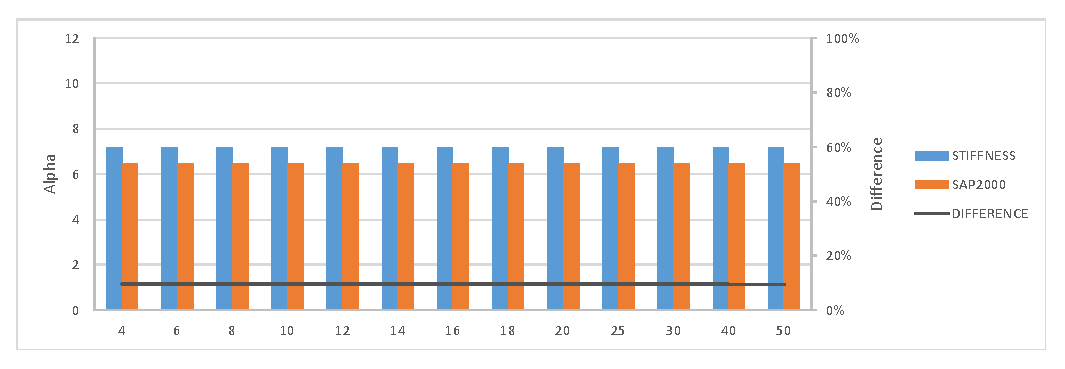
\includegraphics[width=\columnwidth]{images/inkscapeEPS}
\caption{A ``true'' Vector Graph}
\label{inkscapeEPS}
\end{figure}

The procedure followed in obtaining \ref{inkscapeEPS} is as follows:
\begin{enumerate}
\item Print the graph as a PDF file.
\item Open the PDF file in Inkscape.
\item Re-adjust the page size to fit to contents.
\item Save the document in Inkscape as a plain EPS or PDF file. \textbf{Do not} select any options such as \emph{EPS+LaTeX}. Only \emph{Export area is drawing} may be selected.
\item Include epstopdf package in preamble (\texttt{\textbackslash usepackage\{epstopdf\}}) if an EPS file will be used.
\item Use the resultant EPS or PDF file in the document as follows:
\begin{verbatim}
\begin{figure}[htbp]
\centering
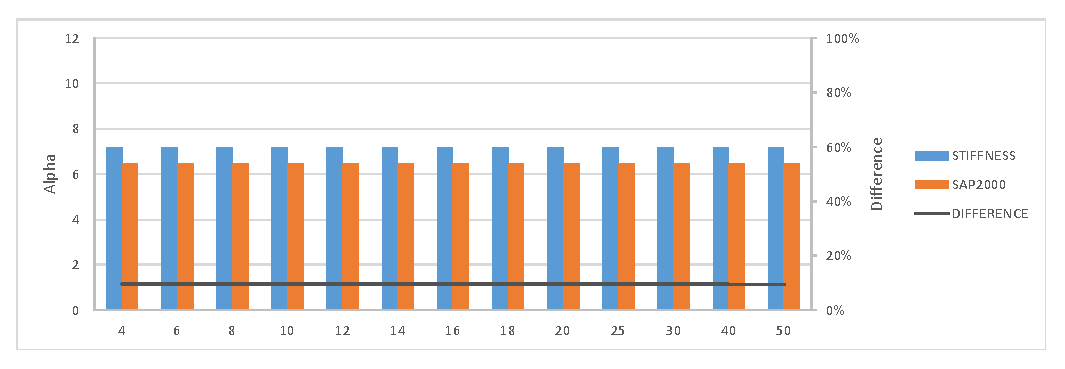
\includegraphics[width=\columnwidth]{images/inkscapeEPS}
\caption{A ``true'' Vector Graph}
\label{inkscapeEPS}
\end{figure}
\end{verbatim}
\end{enumerate}
Please note that if EPS file type will be used, \emph{epstopdf} package will convert these to PDF files with names such as \textsl{\textit{oldFileName-eps-converted-to.pdf}}. Therefore, to eliminate this one extra (though automatic) step, we may select to save PDF from Inkscape directly. In this case, the only reason to fiddle with Inkscape is to adjust the page size of the pdf file, as it will usually be a standard A4 (which will result in very large blank space on top and bottom of the chart). Next approach will overcome this work-around.
\paragraph{Using Custom Size PDF Printing} 
If desired, the use of a second program can be eliminated by doing some extra work on the original software used. The Figure \ref{PDFDirect} is obtained after such a process.
\begin{figure}[htbp]
\centering
\includegraphics[width=\columnwidth]{images/customPDF}
\caption{A Directly Obtained PDF Output}
\label{PDFDirect}
\end{figure}
\\ The algorithm followed in creation of the Excel chart in Figure \ref{PDFDirect} is as follows:
\begin{enumerate}
\item Select the chart in Excel and learn its original dimensions. For this chart, it is 20.04cm x 5.61cm.
\item Press Ctrl+P to show ``Print Dialog'' window. 
\item Click ``Page Setup'', then ``Page'' tab, then ``Options'' button, then ``Layout'' tab, then ``Advanced'' button\footnote{Holy cracker, there should be a shortcut for this!}.
\item In paper size dropdown, select ``PostScript Custom Page Size''.
\item In the newly shown dialog, enter chart dimensions obtained in step 1. \emph{Beware}, these are in mm whereas we learnt them as cm.
\item Close this dialog.
\item In the ``Page Setup'' dialog, set all the margins in the ``Margins'' tab to zero.
\item Print the graph as PDF. 
\item Use the resultant PDF file as follows in \LaTeX:
\begin{verbatim}
\begin{figure}[htbp]
\centering
\includegraphics[width=\columnwidth]{images/customPDF}
\caption{A Directly Obtained PDF Output}
\label{PDFDirect}
\end{figure}
\end{verbatim}
\end{enumerate}
To simplify things and make this approach a 1-click process, I tried to create an Excel add-on that will do steps 1 to 8 automatically. The thing is, it is possible to get dimensions of graph, convert it to cm (as it will be given in PostScript points), make margins zero, change printer to a pdf writer and print the chart. However, the adjustment stated in step 3 and 4 is strictly printer driver-specific. Therefore, it is practically not possible to change these settings in conventional ways (at least I could not find one); .NET native API does not provide support for specifying paper folding, stapling, paper size and other complex actions. In Windows, the DEVMODE data structure contains information about the initialization and environment of a printer or a display device, and it has a \emph{dmDriverExtra} section which contains the number of bytes of private driver-data that follow this structure. It is assumed that the complex settings \textit{live} here in an unknown format. The approach is to get memory dump of DEVMODE structure of a ``configured'' print driver, and before printing we can overwrite the spot of the DEVMODE on memory where this \emph{private data} exists. Obviously it is a very `unorthodox' work-around, and I did not implement this as it will be too much work for a rather simple task. Still, if anyone wants more info, it can be found on internet. 

Another approach is to trim the white space in a PDF file automatically using either \textsl{Inkscape} or \textsc{iTextSharp} (\textsl{GhostScript} itself will work, too). I developed an Excel add-on SaveGraphAsPDF and a standalone app PDFTrimmer for this purpose. 
The second one uses Inkscape and the downside is warnings about group objects in PDF:
\begin{quote}
	PDF inclusion: multiple pdfs with page group included in a single page.
\end{quote}
The reason is, PDF has a feature called `Page Groups' (PDF Reference, section 11.4.7). These describe transparency effects between top-level objects on one page. When pdfTeX (or LuaTeX or XeTeX) includes a page from a PDF, it converts all pages into "Form XObjects" (section 8.10.1). pdfTeX also converts the Page Groups into /Group entries of the XObjects.
The problem now is that Adobe products need also a /Group entry (whose content should not matter) in the /Page object which contains these XObjects to correctly render transparency (this is just needed to select the right rendering engine; the transparency information for the included pages should be taken from these included pages).
pdfTeX will either use the first /Group it encounters when including PDFs or synthesize one when including PNGs with transparency. The warning is triggered when multiple Page Groups are encountered on one page (since the engine will then use the first one encountered and this may not be the "correct" one) and can probably be ignored. As a solution, PDFTrimmer recreates PDF by changing its color space to sRGB using GhostScript. 
\paragraph{matplotlib}
matplotlib is a python 2D plotting library which produces publication quality figures in a variety of hardcopy formats and interactive environments across platforms. matplotlib can be used in python scripts, the python and ipython shell (ala MATLAB or Mathematica), web application servers, and six graphical user interface toolkits.
\paragraph{Generic Mapping Tools (GMT)} Overview
The Generic Mapping Tools, GMT, are an open source collection of tools for manipulating geographic and Cartesian data sets (including filtering, trend fitting, gridding, projecting, etc.) and producing PostScript illustrations ranging from simple x–y plots via contour maps to artificially illuminated surfaces and 3D perspective views. It is released under the GNU Lesser General Public License.
\subsection{Bibliography}
A bibliography item is created within a \texttt{thebibliography} environment, and each entry starts with \emph{\textbackslash bibitem[label]\{marker\}}. The \emph{marker} is then used to cite the resource in within the document: \emph{\textbackslash cite\{marker\}}.

If the \emph{label} option is not used, the entries will get enumerated automatically. The parameter after the \texttt{\textbackslash begin\{thebibliography\}} command defines how much space to reserve for the number of labels; \{99\} tells \LaTeX to expect that none of the bibliography item numbers will be wider than the number 99. 

For larger projects, Bib\TeX program is better suited. It allows to maintain a bibliographic database and then extract the references relevant to things cited in document. 
\end{document}
